\documentclass[]{article}
\usepackage{lmodern}
\usepackage{amssymb,amsmath}
\usepackage{ifxetex,ifluatex}
\usepackage{fixltx2e} % provides \textsubscript
\ifnum 0\ifxetex 1\fi\ifluatex 1\fi=0 % if pdftex
  \usepackage[T1]{fontenc}
  \usepackage[utf8]{inputenc}
\else % if luatex or xelatex
  \ifxetex
    \usepackage{mathspec}
  \else
    \usepackage{fontspec}
  \fi
  \defaultfontfeatures{Ligatures=TeX,Scale=MatchLowercase}
\fi
% use upquote if available, for straight quotes in verbatim environments
\IfFileExists{upquote.sty}{\usepackage{upquote}}{}
% use microtype if available
\IfFileExists{microtype.sty}{%
\usepackage{microtype}
\UseMicrotypeSet[protrusion]{basicmath} % disable protrusion for tt fonts
}{}
\usepackage[margin=1in]{geometry}
\usepackage{hyperref}
\hypersetup{unicode=true,
            pdftitle={R Notebook},
            pdfborder={0 0 0},
            breaklinks=true}
\urlstyle{same}  % don't use monospace font for urls
\usepackage{color}
\usepackage{fancyvrb}
\newcommand{\VerbBar}{|}
\newcommand{\VERB}{\Verb[commandchars=\\\{\}]}
\DefineVerbatimEnvironment{Highlighting}{Verbatim}{commandchars=\\\{\}}
% Add ',fontsize=\small' for more characters per line
\newenvironment{Shaded}{}{}
\newcommand{\KeywordTok}[1]{\textcolor[rgb]{0.00,0.44,0.13}{\textbf{{#1}}}}
\newcommand{\DataTypeTok}[1]{\textcolor[rgb]{0.56,0.13,0.00}{{#1}}}
\newcommand{\DecValTok}[1]{\textcolor[rgb]{0.25,0.63,0.44}{{#1}}}
\newcommand{\BaseNTok}[1]{\textcolor[rgb]{0.25,0.63,0.44}{{#1}}}
\newcommand{\FloatTok}[1]{\textcolor[rgb]{0.25,0.63,0.44}{{#1}}}
\newcommand{\ConstantTok}[1]{\textcolor[rgb]{0.53,0.00,0.00}{{#1}}}
\newcommand{\CharTok}[1]{\textcolor[rgb]{0.25,0.44,0.63}{{#1}}}
\newcommand{\SpecialCharTok}[1]{\textcolor[rgb]{0.25,0.44,0.63}{{#1}}}
\newcommand{\StringTok}[1]{\textcolor[rgb]{0.25,0.44,0.63}{{#1}}}
\newcommand{\VerbatimStringTok}[1]{\textcolor[rgb]{0.25,0.44,0.63}{{#1}}}
\newcommand{\SpecialStringTok}[1]{\textcolor[rgb]{0.73,0.40,0.53}{{#1}}}
\newcommand{\ImportTok}[1]{{#1}}
\newcommand{\CommentTok}[1]{\textcolor[rgb]{0.38,0.63,0.69}{\textit{{#1}}}}
\newcommand{\DocumentationTok}[1]{\textcolor[rgb]{0.73,0.13,0.13}{\textit{{#1}}}}
\newcommand{\AnnotationTok}[1]{\textcolor[rgb]{0.38,0.63,0.69}{\textbf{\textit{{#1}}}}}
\newcommand{\CommentVarTok}[1]{\textcolor[rgb]{0.38,0.63,0.69}{\textbf{\textit{{#1}}}}}
\newcommand{\OtherTok}[1]{\textcolor[rgb]{0.00,0.44,0.13}{{#1}}}
\newcommand{\FunctionTok}[1]{\textcolor[rgb]{0.02,0.16,0.49}{{#1}}}
\newcommand{\VariableTok}[1]{\textcolor[rgb]{0.10,0.09,0.49}{{#1}}}
\newcommand{\ControlFlowTok}[1]{\textcolor[rgb]{0.00,0.44,0.13}{\textbf{{#1}}}}
\newcommand{\OperatorTok}[1]{\textcolor[rgb]{0.40,0.40,0.40}{{#1}}}
\newcommand{\BuiltInTok}[1]{{#1}}
\newcommand{\ExtensionTok}[1]{{#1}}
\newcommand{\PreprocessorTok}[1]{\textcolor[rgb]{0.74,0.48,0.00}{{#1}}}
\newcommand{\AttributeTok}[1]{\textcolor[rgb]{0.49,0.56,0.16}{{#1}}}
\newcommand{\RegionMarkerTok}[1]{{#1}}
\newcommand{\InformationTok}[1]{\textcolor[rgb]{0.38,0.63,0.69}{\textbf{\textit{{#1}}}}}
\newcommand{\WarningTok}[1]{\textcolor[rgb]{0.38,0.63,0.69}{\textbf{\textit{{#1}}}}}
\newcommand{\AlertTok}[1]{\textcolor[rgb]{1.00,0.00,0.00}{\textbf{{#1}}}}
\newcommand{\ErrorTok}[1]{\textcolor[rgb]{1.00,0.00,0.00}{\textbf{{#1}}}}
\newcommand{\NormalTok}[1]{{#1}}
\usepackage{graphicx,grffile}
\makeatletter
\def\maxwidth{\ifdim\Gin@nat@width>\linewidth\linewidth\else\Gin@nat@width\fi}
\def\maxheight{\ifdim\Gin@nat@height>\textheight\textheight\else\Gin@nat@height\fi}
\makeatother
% Scale images if necessary, so that they will not overflow the page
% margins by default, and it is still possible to overwrite the defaults
% using explicit options in \includegraphics[width, height, ...]{}
\setkeys{Gin}{width=\maxwidth,height=\maxheight,keepaspectratio}
\IfFileExists{parskip.sty}{%
\usepackage{parskip}
}{% else
\setlength{\parindent}{0pt}
\setlength{\parskip}{6pt plus 2pt minus 1pt}
}
\setlength{\emergencystretch}{3em}  % prevent overfull lines
\providecommand{\tightlist}{%
  \setlength{\itemsep}{0pt}\setlength{\parskip}{0pt}}
\setcounter{secnumdepth}{0}
% Redefines (sub)paragraphs to behave more like sections
\ifx\paragraph\undefined\else
\let\oldparagraph\paragraph
\renewcommand{\paragraph}[1]{\oldparagraph{#1}\mbox{}}
\fi
\ifx\subparagraph\undefined\else
\let\oldsubparagraph\subparagraph
\renewcommand{\subparagraph}[1]{\oldsubparagraph{#1}\mbox{}}
\fi

%%% Use protect on footnotes to avoid problems with footnotes in titles
\let\rmarkdownfootnote\footnote%
\def\footnote{\protect\rmarkdownfootnote}

%%% Change title format to be more compact
\usepackage{titling}

% Create subtitle command for use in maketitle
\newcommand{\subtitle}[1]{
  \posttitle{
    \begin{center}\large#1\end{center}
    }
}

\setlength{\droptitle}{-2em}
  \title{R Notebook}
  \pretitle{\vspace{\droptitle}\centering\huge}
  \posttitle{\par}
  \author{}
  \preauthor{}\postauthor{}
  \date{}
  \predate{}\postdate{}


\begin{document}
\maketitle

Analysis of equilibrium resonse to power law scaling behaviors,
single-consumer resource case.

\begin{Shaded}
\begin{Highlighting}[]
\KeywordTok{library}\NormalTok{(tidyverse)}
\end{Highlighting}
\end{Shaded}

\begin{Shaded}
\begin{Highlighting}[]
\NormalTok{dat <-}\StringTok{ }\KeywordTok{read_csv}\NormalTok{(}\StringTok{'socio-eco-nw equilibrium-pop-table.csv'}\NormalTok{, }\DataTypeTok{skip =} \DecValTok{6}\NormalTok{) %>%}
\StringTok{  }\KeywordTok{select}\NormalTok{(alpha, beta, }\DataTypeTok{h =} \DecValTok{3}\NormalTok{, }\DataTypeTok{Population =} \DecValTok{12}\NormalTok{) %>%}
\StringTok{  }\KeywordTok{full_join}\NormalTok{((}\KeywordTok{read_csv}\NormalTok{(}\StringTok{'socio-eco-nw equilibrium-bio-table.csv'}\NormalTok{, }\DataTypeTok{skip =} \DecValTok{6}\NormalTok{) %>%}
\StringTok{  }\KeywordTok{select}\NormalTok{(alpha, beta, }\DataTypeTok{Biomass =} \DecValTok{12}\NormalTok{))) %>%}
\StringTok{  }\KeywordTok{mutate}\NormalTok{(}\DataTypeTok{Welfare =} \NormalTok{Biomass *}\StringTok{ }\NormalTok{h *}\StringTok{ }\NormalTok{Population^(beta}\DecValTok{-1}\NormalTok{)) %>%}
\StringTok{  }\KeywordTok{select}\NormalTok{(-h)}
\end{Highlighting}
\end{Shaded}

Find equilibrium values

\begin{Shaded}
\begin{Highlighting}[]
\NormalTok{dat %>%}\StringTok{ }\KeywordTok{filter}\NormalTok{(alpha ==}\StringTok{ }\DecValTok{1} \NormalTok{&}\StringTok{ }\NormalTok{beta ==}\StringTok{ }\DecValTok{1}\NormalTok{) %>%}\StringTok{ }\KeywordTok{select}\NormalTok{(}\DecValTok{3}\NormalTok{:}\DecValTok{5}\NormalTok{)}
\end{Highlighting}
\end{Shaded}

\begin{verbatim}
## # A tibble: 1 × 3
##   Population Biomass Welfare
##        <dbl>   <dbl>   <dbl>
## 1      60000     0.4   4e-07
\end{verbatim}

Normalize data using equilibrium values

\begin{Shaded}
\begin{Highlighting}[]
\NormalTok{dat.norm <-}\StringTok{ }\NormalTok{dat %>%}\StringTok{ }
\StringTok{  }\KeywordTok{mutate}\NormalTok{(}\DataTypeTok{Population =} \NormalTok{Population /}\StringTok{ }\DecValTok{60000}\NormalTok{, }\DataTypeTok{Biomass =} \NormalTok{Biomass /}\StringTok{ }\NormalTok{.}\DecValTok{4}\NormalTok{, }\DataTypeTok{Welfare =} \NormalTok{Welfare /}\StringTok{ }\FloatTok{4e-07}\NormalTok{)}
\end{Highlighting}
\end{Shaded}

\begin{Shaded}
\begin{Highlighting}[]
\NormalTok{dat.norm %>%}\StringTok{ }\KeywordTok{gather}\NormalTok{(variable, value, Population:Welfare) %>%}
\StringTok{  }\KeywordTok{ggplot}\NormalTok{(}\KeywordTok{aes}\NormalTok{(alpha, beta, }\DataTypeTok{fill =} \NormalTok{value)) +}
\StringTok{    }\KeywordTok{facet_wrap}\NormalTok{(~variable) +}
\StringTok{    }\KeywordTok{geom_raster}\NormalTok{(}\DataTypeTok{interpolate =} \NormalTok{T) +}
\StringTok{    }\KeywordTok{labs}\NormalTok{(}\DataTypeTok{title =} \StringTok{'Equilibrium sensitivity to power law scaling'}\NormalTok{, }\DataTypeTok{subtitle =} \KeywordTok{expression}\NormalTok{(}\StringTok{'All values normalized to '} \NormalTok{*}\StringTok{ }\NormalTok{alpha *}\StringTok{' = '} \NormalTok{*}\StringTok{ }\NormalTok{beta *}\StringTok{ ' = 1'}\NormalTok{), }\DataTypeTok{x =} \KeywordTok{expression}\NormalTok{(alpha), }\DataTypeTok{y =} \KeywordTok{expression}\NormalTok{(beta)) +}
\StringTok{    }\KeywordTok{scale_fill_distiller}\NormalTok{(}\DataTypeTok{name =} \StringTok{'Value at }\CharTok{\textbackslash{}n}\StringTok{equilibrium'}\NormalTok{, }\DataTypeTok{palette =} \StringTok{'Spectral'}\NormalTok{, }\DataTypeTok{guide =} \StringTok{'legend'}\NormalTok{, }\DataTypeTok{breaks =} \KeywordTok{c}\NormalTok{(.}\DecValTok{1}\NormalTok{,}\DecValTok{3}\NormalTok{),}\DataTypeTok{labels =} \KeywordTok{c}\NormalTok{(}\StringTok{'Low'}\NormalTok{, }\StringTok{'High'}\NormalTok{)) +}
\StringTok{    }\KeywordTok{scale_x_continuous}\NormalTok{(}\DataTypeTok{breaks =} \KeywordTok{c}\NormalTok{(.}\DecValTok{9}\NormalTok{, }\DecValTok{1}\NormalTok{, }\FloatTok{1.1}\NormalTok{)) +}
\StringTok{    }\KeywordTok{coord_equal}\NormalTok{() +}
\StringTok{    }\KeywordTok{theme_minimal}\NormalTok{()}
\end{Highlighting}
\end{Shaded}

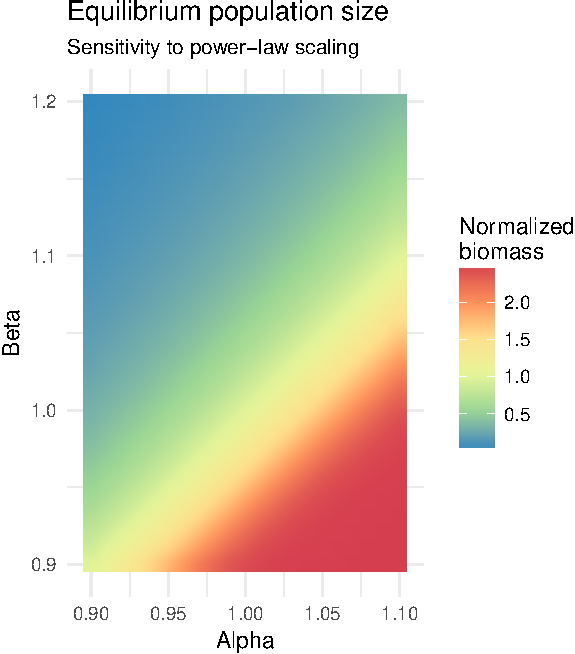
\includegraphics{eq_pop_files/figure-latex/unnamed-chunk-5-1.pdf} In
natural language, resource biomass is highest when higher population
leads to declining marignal returns to harvest

\subsection{alpha beta plots}\label{alpha-beta-plots}

plots of how different exponents effect population size

\begin{Shaded}
\begin{Highlighting}[]
\NormalTok{dat <-}\StringTok{ }\KeywordTok{data_frame}\NormalTok{(}\DataTypeTok{n =} \DecValTok{1}\NormalTok{:}\DecValTok{1000}\NormalTok{) %>%}
\StringTok{  }\KeywordTok{mutate}\NormalTok{(}\StringTok{'0.8'} \NormalTok{=}\StringTok{ }\NormalTok{n^.}\DecValTok{8}\NormalTok{,}
         \StringTok{'0.9'} \NormalTok{=}\StringTok{ }\NormalTok{n^.}\DecValTok{9}\NormalTok{,}
         \StringTok{'1.0'} \NormalTok{=}\StringTok{ }\NormalTok{n^}\DecValTok{1}\NormalTok{,}
         \StringTok{'1.1'} \NormalTok{=}\StringTok{ }\NormalTok{n^}\FloatTok{1.1}\NormalTok{,}
         \StringTok{'1.2'} \NormalTok{=}\StringTok{ }\NormalTok{n^}\FloatTok{1.2}\NormalTok{) %>%}
\StringTok{  }\KeywordTok{gather}\NormalTok{(key, value, }\DecValTok{2}\NormalTok{:}\DecValTok{6}\NormalTok{)}

\KeywordTok{ggplot}\NormalTok{(dat, }\KeywordTok{aes}\NormalTok{(}\DataTypeTok{x =} \NormalTok{n, }\DataTypeTok{y =} \NormalTok{value, }\DataTypeTok{color =} \NormalTok{key)) +}
\StringTok{  }\KeywordTok{geom_line}\NormalTok{(}\DataTypeTok{size =} \FloatTok{1.2}\NormalTok{) +}
\StringTok{  }\KeywordTok{labs}\NormalTok{(}\DataTypeTok{title =} \StringTok{'Impact of power law scaling'}\NormalTok{, }\DataTypeTok{subtitle =} \StringTok{'Superlinear scaling in red, sublinear scaling in blue'}\NormalTok{, }\DataTypeTok{x =} \StringTok{'Population'}\NormalTok{, }\DataTypeTok{y =} \StringTok{'Value'}\NormalTok{) +}
\StringTok{  }\KeywordTok{scale_color_brewer}\NormalTok{(}\DataTypeTok{palette =} \StringTok{'RdYlBu'}\NormalTok{, }\DataTypeTok{direction =} \NormalTok{-}\DecValTok{1}\NormalTok{, }\DataTypeTok{name =} \StringTok{'Scaling }\CharTok{\textbackslash{}n}\StringTok{parameter'}\NormalTok{) +}
\StringTok{  }\KeywordTok{theme_minimal}\NormalTok{()}
\end{Highlighting}
\end{Shaded}

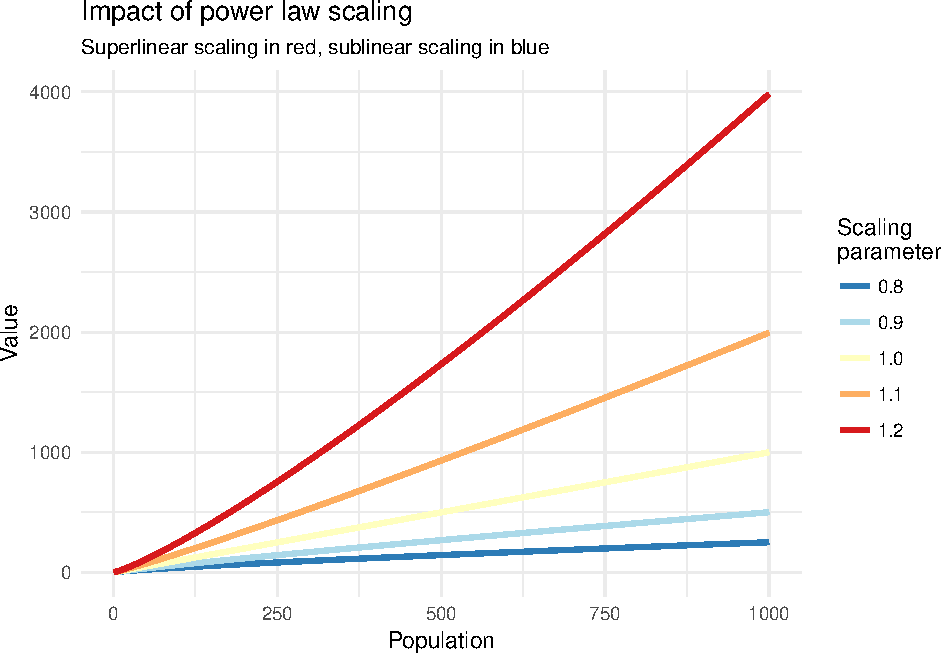
\includegraphics{eq_pop_files/figure-latex/unnamed-chunk-6-1.pdf}

\subsection{network plots}\label{network-plots}

simple plots of networks

\begin{Shaded}
\begin{Highlighting}[]
\KeywordTok{library}\NormalTok{(ggraph)}
\KeywordTok{library}\NormalTok{(igraph)}
\end{Highlighting}
\end{Shaded}

\begin{verbatim}
## 
## Attaching package: 'igraph'
\end{verbatim}

\begin{verbatim}
## The following objects are masked from 'package:dplyr':
## 
##     %>%, as_data_frame, groups, union
\end{verbatim}

\begin{verbatim}
## The following objects are masked from 'package:purrr':
## 
##     %>%, compose, simplify
\end{verbatim}

\begin{verbatim}
## The following objects are masked from 'package:tidyr':
## 
##     %>%, crossing
\end{verbatim}

\begin{verbatim}
## The following object is masked from 'package:tibble':
## 
##     as_data_frame
\end{verbatim}

\begin{verbatim}
## The following objects are masked from 'package:stats':
## 
##     decompose, spectrum
\end{verbatim}

\begin{verbatim}
## The following object is masked from 'package:base':
## 
##     union
\end{verbatim}

\begin{Shaded}
\begin{Highlighting}[]
\NormalTok{vert.dat <-}\StringTok{ }\KeywordTok{data_frame}\NormalTok{(}\DataTypeTok{names =} \DecValTok{1}\NormalTok{:}\DecValTok{6}\NormalTok{, }\DataTypeTok{Type =} \KeywordTok{c}\NormalTok{(}\StringTok{'City'}\NormalTok{, }\StringTok{'City'}\NormalTok{, }\StringTok{'City'}\NormalTok{, }\StringTok{'Resource'}\NormalTok{, }\StringTok{'Resource'}\NormalTok{, }\StringTok{'Resource'}\NormalTok{))}

\NormalTok{net <-}\StringTok{ }\KeywordTok{data_frame}\NormalTok{(}\DataTypeTok{from =} \KeywordTok{c}\NormalTok{(}\DecValTok{1}\NormalTok{, }\DecValTok{1}\NormalTok{, }\DecValTok{2}\NormalTok{, }\DecValTok{3}\NormalTok{, }\DecValTok{1}\NormalTok{, }\DecValTok{1}\NormalTok{, }\DecValTok{2}\NormalTok{, }\DecValTok{3}\NormalTok{, }\DecValTok{1}\NormalTok{, }\DecValTok{1}\NormalTok{, }\DecValTok{1}\NormalTok{, }\DecValTok{2}\NormalTok{, }\DecValTok{3}\NormalTok{, }\DecValTok{2}\NormalTok{, }\DecValTok{1}\NormalTok{, }\DecValTok{1}\NormalTok{, }\DecValTok{2}\NormalTok{, }\DecValTok{3}\NormalTok{, }\DecValTok{1}\NormalTok{),}
           \DataTypeTok{to =} \KeywordTok{c}\NormalTok{(}\DecValTok{4}\NormalTok{, }\DecValTok{5}\NormalTok{, }\DecValTok{5}\NormalTok{, }\DecValTok{6}\NormalTok{, }\DecValTok{4}\NormalTok{, }\DecValTok{5}\NormalTok{, }\DecValTok{5}\NormalTok{, }\DecValTok{6}\NormalTok{, }\DecValTok{2}\NormalTok{, }\DecValTok{4}\NormalTok{, }\DecValTok{5}\NormalTok{, }\DecValTok{5}\NormalTok{, }\DecValTok{6}\NormalTok{, }\DecValTok{3}\NormalTok{, }\DecValTok{4}\NormalTok{, }\DecValTok{5}\NormalTok{, }\DecValTok{5}\NormalTok{, }\DecValTok{6}\NormalTok{, }\DecValTok{3}\NormalTok{), }
           \DataTypeTok{structure =} \KeywordTok{c}\NormalTok{(}\DecValTok{1}\NormalTok{, }\DecValTok{1}\NormalTok{, }\DecValTok{1}\NormalTok{, }\DecValTok{1}\NormalTok{, }\DecValTok{2}\NormalTok{, }\DecValTok{2}\NormalTok{, }\DecValTok{2}\NormalTok{, }\DecValTok{2}\NormalTok{, }\DecValTok{2}\NormalTok{, }\DecValTok{3}\NormalTok{, }\DecValTok{3}\NormalTok{, }\DecValTok{3}\NormalTok{, }\DecValTok{3}\NormalTok{, }\DecValTok{3}\NormalTok{, }\DecValTok{4}\NormalTok{, }\DecValTok{4}\NormalTok{, }\DecValTok{4}\NormalTok{, }\DecValTok{4}\NormalTok{, }\DecValTok{4}\NormalTok{),}
           \DataTypeTok{Link =} \KeywordTok{c}\NormalTok{(}\StringTok{'City-Resource'}\NormalTok{, }\StringTok{'City-Resource'}\NormalTok{, }\StringTok{'City-Resource'}\NormalTok{, }\StringTok{'City-Resource'}\NormalTok{, }\StringTok{'City-Resource'}\NormalTok{, }\StringTok{'City-Resource'}\NormalTok{, }\StringTok{'City-Resource'}\NormalTok{, }\StringTok{'City-Resource'}\NormalTok{, }\StringTok{'City-City'}\NormalTok{, }\StringTok{'City-Resource'}\NormalTok{, }\StringTok{'City-Resource'}\NormalTok{, }\StringTok{'City-Resource'}\NormalTok{, }\StringTok{'City-Resource'}\NormalTok{, }\StringTok{'City-City'}\NormalTok{, }\StringTok{'City-Resource'}\NormalTok{, }\StringTok{'City-Resource'}\NormalTok{, }\StringTok{'City-Resource'}\NormalTok{, }\StringTok{'City-Resource'}\NormalTok{, }\StringTok{'City-City'}\NormalTok{)) %>%}\StringTok{ }\KeywordTok{graph_from_data_frame}\NormalTok{(}\DataTypeTok{directed =} \NormalTok{F, vert.dat)}
\end{Highlighting}
\end{Shaded}

\begin{Shaded}
\begin{Highlighting}[]
\KeywordTok{ggraph}\NormalTok{(net, }\StringTok{'kk'}\NormalTok{) +}
\StringTok{  }\KeywordTok{geom_edge_fan}\NormalTok{(}\KeywordTok{aes}\NormalTok{(}\DataTypeTok{color =} \NormalTok{Link)) +}
\StringTok{  }\KeywordTok{geom_node_point}\NormalTok{(}\KeywordTok{aes}\NormalTok{(}\DataTypeTok{color =} \NormalTok{Type), }\DataTypeTok{size =} \DecValTok{5}\NormalTok{) +}
\StringTok{  }\KeywordTok{facet_edges}\NormalTok{(~structure) +}
\StringTok{  }\KeywordTok{labs}\NormalTok{(}\DataTypeTok{title =} \StringTok{'Potential social-ecological connectivity structures'}\NormalTok{, }\DataTypeTok{subtitle =} \KeywordTok{expression}\NormalTok{(}\StringTok{'Under different parameterizations of '} \NormalTok{*}\StringTok{ }\KeywordTok{bold}\NormalTok{(xi))) +}
\StringTok{  }\KeywordTok{coord_equal}\NormalTok{() +}
\StringTok{  }\KeywordTok{theme_void}\NormalTok{() +}
\StringTok{  }\KeywordTok{theme}\NormalTok{(}\DataTypeTok{panel.spacing =} \KeywordTok{unit}\NormalTok{(}\DecValTok{3}\NormalTok{, }\StringTok{"lines"}\NormalTok{), }\DataTypeTok{strip.text =} \KeywordTok{element_blank}\NormalTok{())}
\end{Highlighting}
\end{Shaded}

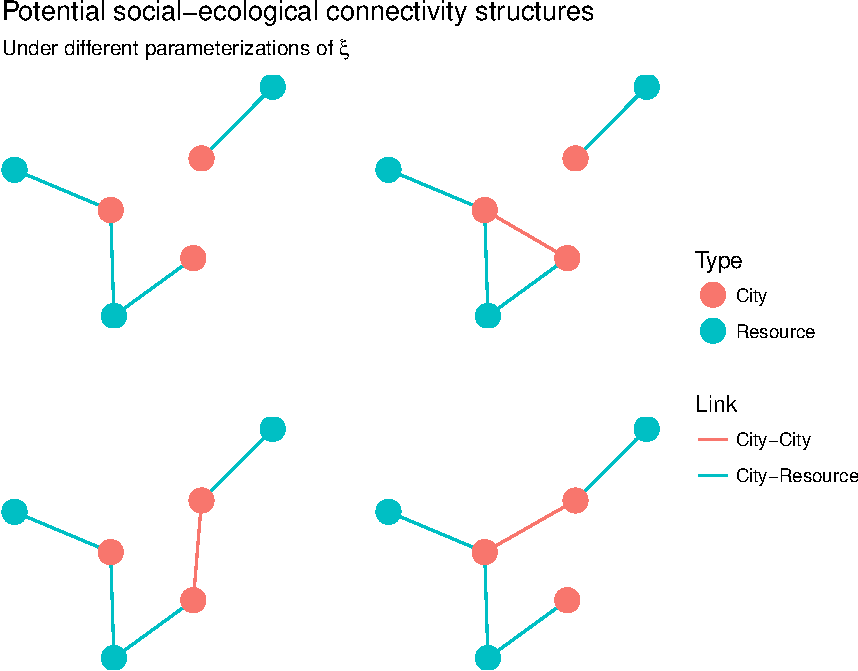
\includegraphics{eq_pop_files/figure-latex/connectivity-1.pdf}

\begin{Shaded}
\begin{Highlighting}[]
\CommentTok{#dat %>% filter(alpha == .9 & beta == 1.2) %>% select(3:5)}
\end{Highlighting}
\end{Shaded}

\begin{Shaded}
\begin{Highlighting}[]
\NormalTok{n1.vert <-}\StringTok{ }\KeywordTok{data_frame}\NormalTok{(}\DataTypeTok{names =} \DecValTok{1}\NormalTok{:}\DecValTok{6}\NormalTok{, }
                      \DataTypeTok{Type =} \KeywordTok{c}\NormalTok{(}\StringTok{'City'}\NormalTok{, }\StringTok{'City'}\NormalTok{, }\StringTok{'City'}\NormalTok{, }\StringTok{'Resource'}\NormalTok{, }\StringTok{'Resource'}\NormalTok{, }\StringTok{'Resource'}\NormalTok{),}
                      \DataTypeTok{pop =} \KeywordTok{c}\NormalTok{(}\KeywordTok{c}\NormalTok{(}\DecValTok{14540}\NormalTok{, }\DecValTok{0}\NormalTok{, }\DecValTok{14401}\NormalTok{)/}\FloatTok{14400.75}\NormalTok{, }\KeywordTok{c}\NormalTok{(.}\DecValTok{0113}\NormalTok{,.}\DecValTok{0113}\NormalTok{,.}\DecValTok{0226}\NormalTok{)/.}\DecValTok{0226227}\NormalTok{))}

\NormalTok{n1 <-}\StringTok{ }\KeywordTok{data_frame}\NormalTok{(}\DataTypeTok{from =} \KeywordTok{c}\NormalTok{(}\DecValTok{1}\NormalTok{, }\DecValTok{1}\NormalTok{, }\DecValTok{2}\NormalTok{, }\DecValTok{3}\NormalTok{),}
           \DataTypeTok{to =} \KeywordTok{c}\NormalTok{(}\DecValTok{4}\NormalTok{, }\DecValTok{5}\NormalTok{, }\DecValTok{5}\NormalTok{, }\DecValTok{6}\NormalTok{),}
           \DataTypeTok{Link =} \KeywordTok{c}\NormalTok{(}\StringTok{'City-Resource'}\NormalTok{, }\StringTok{'City-Resource'}\NormalTok{, }\StringTok{'City-Resource'}\NormalTok{, }\StringTok{'City-Resource'}\NormalTok{)) %>%}\StringTok{ }\KeywordTok{graph_from_data_frame}\NormalTok{(}\DataTypeTok{directed =} \NormalTok{F, n1.vert)}

\NormalTok{orig.layout <-}\StringTok{ }\KeywordTok{create_layout}\NormalTok{(net, }\StringTok{'kk'}\NormalTok{) %>%}
\StringTok{  }\KeywordTok{select}\NormalTok{(x:y)}

\NormalTok{n1.layout <-}\StringTok{ }\KeywordTok{create_layout}\NormalTok{(n1, }\StringTok{'kk'}\NormalTok{)}
\NormalTok{n1.layout[,}\DecValTok{1}\NormalTok{] <-}\StringTok{  }\NormalTok{orig.layout[,}\DecValTok{1}\NormalTok{] }
\NormalTok{n1.layout[,}\DecValTok{2}\NormalTok{] <-}\StringTok{ }\NormalTok{orig.layout[,}\DecValTok{2}\NormalTok{]}

\NormalTok{n1.plt <-}\StringTok{ }\KeywordTok{ggraph}\NormalTok{(n1.layout, }\DataTypeTok{layout =} \NormalTok{my.layout) +}
\StringTok{  }\KeywordTok{geom_edge_fan}\NormalTok{(}\DataTypeTok{colour =} \StringTok{'#00BFC4'}\NormalTok{) +}
\StringTok{  }\KeywordTok{geom_node_point}\NormalTok{(}\KeywordTok{aes}\NormalTok{(}\DataTypeTok{color =} \NormalTok{Type, }\DataTypeTok{size =} \NormalTok{pop)) +}
\StringTok{  }\KeywordTok{scale_size_area}\NormalTok{() +}
\StringTok{  }\KeywordTok{coord_equal}\NormalTok{() +}
\StringTok{  }\KeywordTok{theme_void}\NormalTok{() +}
\StringTok{  }\KeywordTok{theme}\NormalTok{(}\DataTypeTok{legend.position =} \StringTok{'none'}\NormalTok{)}
\end{Highlighting}
\end{Shaded}

\begin{Shaded}
\begin{Highlighting}[]
\NormalTok{n2.vert <-}\StringTok{ }\KeywordTok{data_frame}\NormalTok{(}\DataTypeTok{names =} \DecValTok{1}\NormalTok{:}\DecValTok{6}\NormalTok{, }
                      \DataTypeTok{Type =} \KeywordTok{c}\NormalTok{(}\StringTok{'City'}\NormalTok{, }\StringTok{'City'}\NormalTok{, }\StringTok{'City'}\NormalTok{, }\StringTok{'Resource'}\NormalTok{, }\StringTok{'Resource'}\NormalTok{, }\StringTok{'Resource'}\NormalTok{),}
                      \DataTypeTok{pop =} \KeywordTok{c}\NormalTok{(}\KeywordTok{c}\NormalTok{(}\DecValTok{14409}\NormalTok{, }\DecValTok{565}\NormalTok{, }\DecValTok{14401}\NormalTok{)/}\FloatTok{14400.75}\NormalTok{, }\KeywordTok{c}\NormalTok{(.}\DecValTok{0219}\NormalTok{, .}\DecValTok{0119}\NormalTok{,.}\DecValTok{0226}\NormalTok{)/.}\DecValTok{0226227}\NormalTok{))}

\NormalTok{n2 <-}\StringTok{ }\KeywordTok{data_frame}\NormalTok{(}\DataTypeTok{from =} \KeywordTok{c}\NormalTok{(}\DecValTok{1}\NormalTok{, }\DecValTok{1}\NormalTok{, }\DecValTok{2}\NormalTok{, }\DecValTok{3}\NormalTok{, }\DecValTok{1}\NormalTok{),}
           \DataTypeTok{to =} \KeywordTok{c}\NormalTok{(}\DecValTok{4}\NormalTok{, }\DecValTok{5}\NormalTok{, }\DecValTok{5}\NormalTok{, }\DecValTok{6}\NormalTok{, }\DecValTok{2}\NormalTok{),}
           \DataTypeTok{Link =} \KeywordTok{c}\NormalTok{(}\StringTok{'City-Resource'}\NormalTok{, }\StringTok{'City-Resource'}\NormalTok{, }\StringTok{'City-Resource'}\NormalTok{, }\StringTok{'City-Resource'}\NormalTok{, }\StringTok{'City-City'}\NormalTok{)) %>%}\StringTok{ }\KeywordTok{graph_from_data_frame}\NormalTok{(}\DataTypeTok{directed =} \NormalTok{F, n2.vert)}

\NormalTok{n2.layout <-}\StringTok{ }\KeywordTok{create_layout}\NormalTok{(n2, }\StringTok{'kk'}\NormalTok{)}
\NormalTok{n2.layout[,}\DecValTok{1}\NormalTok{] <-}\StringTok{  }\NormalTok{orig.layout[,}\DecValTok{1}\NormalTok{] }
\NormalTok{n2.layout[,}\DecValTok{2}\NormalTok{] <-}\StringTok{ }\NormalTok{orig.layout[,}\DecValTok{2}\NormalTok{]}

\NormalTok{n2.plt <-}\StringTok{ }\KeywordTok{ggraph}\NormalTok{(n2.layout) +}
\StringTok{  }\KeywordTok{geom_edge_fan}\NormalTok{(}\KeywordTok{aes}\NormalTok{(}\DataTypeTok{color =} \NormalTok{Link)) +}
\StringTok{  }\KeywordTok{geom_node_point}\NormalTok{(}\KeywordTok{aes}\NormalTok{(}\DataTypeTok{color =} \NormalTok{Type, }\DataTypeTok{size =} \NormalTok{pop)) +}
\StringTok{  }\KeywordTok{scale_size_area}\NormalTok{() +}
\StringTok{  }\KeywordTok{coord_equal}\NormalTok{() +}
\StringTok{  }\KeywordTok{theme_void}\NormalTok{() +}
\StringTok{  }\KeywordTok{theme}\NormalTok{(}\DataTypeTok{legend.position =} \StringTok{'none'}\NormalTok{)}
\end{Highlighting}
\end{Shaded}

\begin{Shaded}
\begin{Highlighting}[]
\NormalTok{n3.vert <-}\StringTok{ }\KeywordTok{data_frame}\NormalTok{(}\DataTypeTok{names =} \DecValTok{1}\NormalTok{:}\DecValTok{6}\NormalTok{, }
                      \DataTypeTok{Type =} \KeywordTok{c}\NormalTok{(}\StringTok{'City'}\NormalTok{, }\StringTok{'City'}\NormalTok{, }\StringTok{'City'}\NormalTok{, }\StringTok{'Resource'}\NormalTok{, }\StringTok{'Resource'}\NormalTok{, }\StringTok{'Resource'}\NormalTok{),}
                      \DataTypeTok{pop =} \KeywordTok{c}\NormalTok{(}\KeywordTok{c}\NormalTok{(}\DecValTok{14423}\NormalTok{, }\DecValTok{540}\NormalTok{, }\DecValTok{14387}\NormalTok{)/}\FloatTok{14400.75}\NormalTok{, }\KeywordTok{c}\NormalTok{(.}\DecValTok{0208}\NormalTok{, .}\DecValTok{0018}\NormalTok{, .}\DecValTok{0238}\NormalTok{)/.}\DecValTok{0226227}\NormalTok{))}

\NormalTok{n3 <-}\StringTok{ }\KeywordTok{data_frame}\NormalTok{(}\DataTypeTok{from =} \KeywordTok{c}\NormalTok{(}\DecValTok{1}\NormalTok{, }\DecValTok{1}\NormalTok{, }\DecValTok{2}\NormalTok{, }\DecValTok{3}\NormalTok{, }\DecValTok{2}\NormalTok{),}
           \DataTypeTok{to =} \KeywordTok{c}\NormalTok{(}\DecValTok{4}\NormalTok{, }\DecValTok{5}\NormalTok{, }\DecValTok{5}\NormalTok{, }\DecValTok{6}\NormalTok{, }\DecValTok{3}\NormalTok{),}
           \DataTypeTok{Link =} \KeywordTok{c}\NormalTok{(}\StringTok{'City-Resource'}\NormalTok{, }\StringTok{'City-Resource'}\NormalTok{, }\StringTok{'City-Resource'}\NormalTok{, }\StringTok{'City-Resource'}\NormalTok{, }\StringTok{'City-City'}\NormalTok{)) %>%}\StringTok{ }\KeywordTok{graph_from_data_frame}\NormalTok{(}\DataTypeTok{directed =} \NormalTok{F, n3.vert)}

\NormalTok{n3.layout <-}\StringTok{ }\KeywordTok{create_layout}\NormalTok{(n3, }\StringTok{'kk'}\NormalTok{)}
\NormalTok{n3.layout[,}\DecValTok{1}\NormalTok{] <-}\StringTok{  }\NormalTok{orig.layout[,}\DecValTok{1}\NormalTok{] }
\NormalTok{n3.layout[,}\DecValTok{2}\NormalTok{] <-}\StringTok{ }\NormalTok{orig.layout[,}\DecValTok{2}\NormalTok{]}

\NormalTok{n3.plt <-}\StringTok{ }\KeywordTok{ggraph}\NormalTok{(n3.layout) +}
\StringTok{  }\KeywordTok{geom_edge_fan}\NormalTok{(}\KeywordTok{aes}\NormalTok{(}\DataTypeTok{color =} \NormalTok{Link)) +}
\StringTok{  }\KeywordTok{geom_node_point}\NormalTok{(}\KeywordTok{aes}\NormalTok{(}\DataTypeTok{color =} \NormalTok{Type, }\DataTypeTok{size =} \NormalTok{pop)) +}
\StringTok{  }\KeywordTok{scale_size_area}\NormalTok{() +}
\StringTok{  }\KeywordTok{coord_equal}\NormalTok{() +}
\StringTok{  }\KeywordTok{theme_void}\NormalTok{() +}
\StringTok{  }\KeywordTok{theme}\NormalTok{(}\DataTypeTok{legend.position =} \StringTok{'none'}\NormalTok{)}
\end{Highlighting}
\end{Shaded}

\begin{Shaded}
\begin{Highlighting}[]
\NormalTok{n4.vert <-}\StringTok{ }\KeywordTok{data_frame}\NormalTok{(}\DataTypeTok{names =} \DecValTok{1}\NormalTok{:}\DecValTok{6}\NormalTok{, }
                      \DataTypeTok{Type =} \KeywordTok{c}\NormalTok{(}\StringTok{'City'}\NormalTok{, }\StringTok{'City'}\NormalTok{, }\StringTok{'City'}\NormalTok{, }\StringTok{'Resource'}\NormalTok{, }\StringTok{'Resource'}\NormalTok{, }\StringTok{'Resource'}\NormalTok{),}
                      \DataTypeTok{pop =} \KeywordTok{c}\NormalTok{(}\KeywordTok{c}\NormalTok{(}\DecValTok{14539}\NormalTok{, }\DecValTok{0}\NormalTok{, }\DecValTok{14402}\NormalTok{)/}\FloatTok{14400.75}\NormalTok{, }\KeywordTok{c}\NormalTok{(.}\DecValTok{0113}\NormalTok{, .}\DecValTok{0113}\NormalTok{, .}\DecValTok{0225}\NormalTok{)/.}\DecValTok{0226227}\NormalTok{))}

\NormalTok{n4 <-}\StringTok{ }\KeywordTok{data_frame}\NormalTok{(}\DataTypeTok{from =} \KeywordTok{c}\NormalTok{(}\DecValTok{1}\NormalTok{, }\DecValTok{1}\NormalTok{, }\DecValTok{2}\NormalTok{, }\DecValTok{3}\NormalTok{, }\DecValTok{1}\NormalTok{),}
           \DataTypeTok{to =} \KeywordTok{c}\NormalTok{(}\DecValTok{4}\NormalTok{, }\DecValTok{5}\NormalTok{, }\DecValTok{5}\NormalTok{, }\DecValTok{6}\NormalTok{, }\DecValTok{3}\NormalTok{),}
           \DataTypeTok{Link =} \KeywordTok{c}\NormalTok{(}\StringTok{'City-Resource'}\NormalTok{, }\StringTok{'City-Resource'}\NormalTok{, }\StringTok{'City-Resource'}\NormalTok{, }\StringTok{'City-Resource'}\NormalTok{, }\StringTok{'City-City'}\NormalTok{)) %>%}\StringTok{ }\KeywordTok{graph_from_data_frame}\NormalTok{(}\DataTypeTok{directed =} \NormalTok{F, n4.vert)}

\NormalTok{n4.layout <-}\StringTok{ }\KeywordTok{create_layout}\NormalTok{(n4, }\StringTok{'kk'}\NormalTok{)}
\NormalTok{n4.layout[,}\DecValTok{1}\NormalTok{] <-}\StringTok{  }\NormalTok{orig.layout[,}\DecValTok{1}\NormalTok{] }
\NormalTok{n4.layout[,}\DecValTok{2}\NormalTok{] <-}\StringTok{ }\NormalTok{orig.layout[,}\DecValTok{2}\NormalTok{]}

\NormalTok{n4.plt <-}\StringTok{ }\KeywordTok{ggraph}\NormalTok{(n4.layout) +}
\StringTok{  }\KeywordTok{geom_edge_fan}\NormalTok{(}\KeywordTok{aes}\NormalTok{(}\DataTypeTok{color =} \NormalTok{Link)) +}
\StringTok{  }\KeywordTok{geom_node_point}\NormalTok{(}\KeywordTok{aes}\NormalTok{(}\DataTypeTok{color =} \NormalTok{Type, }\DataTypeTok{size =} \NormalTok{pop)) +}
\StringTok{  }\KeywordTok{scale_size_area}\NormalTok{() +}
\StringTok{  }\KeywordTok{coord_equal}\NormalTok{() +}
\StringTok{  }\KeywordTok{theme_void}\NormalTok{() +}
\StringTok{  }\KeywordTok{theme}\NormalTok{(}\DataTypeTok{legend.position =} \StringTok{'none'}\NormalTok{)}
\end{Highlighting}
\end{Shaded}

\begin{Shaded}
\begin{Highlighting}[]
\KeywordTok{library}\NormalTok{(gridExtra)}
\end{Highlighting}
\end{Shaded}

\begin{verbatim}
## 
## Attaching package: 'gridExtra'
\end{verbatim}

\begin{verbatim}
## The following object is masked from 'package:dplyr':
## 
##     combine
\end{verbatim}

\begin{Shaded}
\begin{Highlighting}[]
\KeywordTok{grid.arrange}\NormalTok{(n1.plt, n2.plt, n3.plt, n4.plt)}
\end{Highlighting}
\end{Shaded}

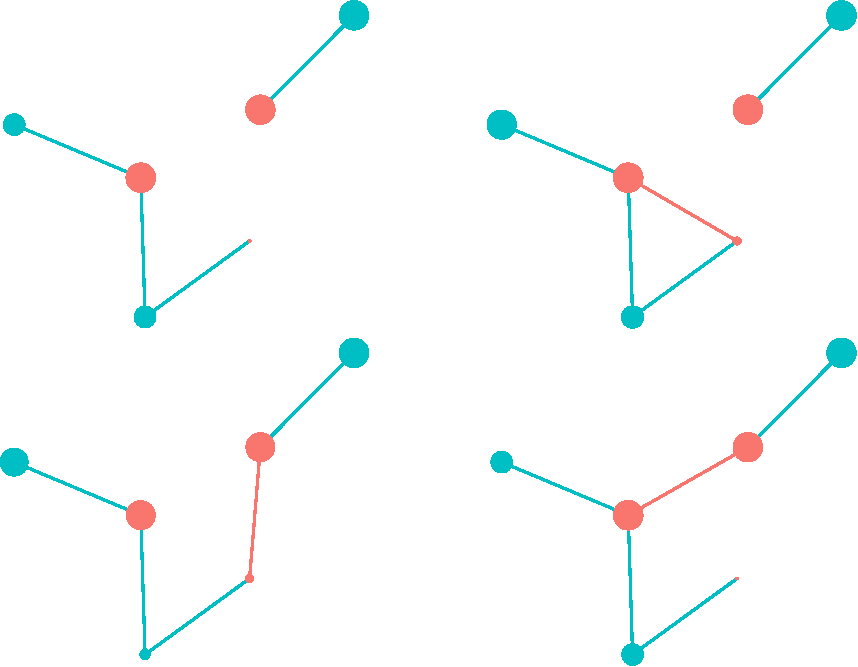
\includegraphics{eq_pop_files/figure-latex/unnamed-chunk-14-1.pdf}

\begin{Shaded}
\begin{Highlighting}[]
\NormalTok{gg_color_hue <-}\StringTok{ }\NormalTok{function(n)\{}
  \NormalTok{hues =}\StringTok{ }\KeywordTok{seq}\NormalTok{(}\DecValTok{15}\NormalTok{, }\DecValTok{375}\NormalTok{, }\DataTypeTok{length =} \NormalTok{n}\DecValTok{+1}\NormalTok{)}
  \KeywordTok{hcl}\NormalTok{(}\DataTypeTok{h =} \NormalTok{hues, }\DataTypeTok{l =} \DecValTok{65}\NormalTok{, }\DataTypeTok{c =} \DecValTok{100}\NormalTok{)[}\DecValTok{1}\NormalTok{:n]}
\NormalTok{\}}
\KeywordTok{gg_color_hue}\NormalTok{(}\DecValTok{2}\NormalTok{)}
\end{Highlighting}
\end{Shaded}

\begin{verbatim}
## [1] "#F8766D" "#00BFC4"
\end{verbatim}


\end{document}
